%----------------------------------------------------------------------------
\chapter{\AudioOverIp}
%----------------------------------------------------------------------------
\section{Bevezetés az Audio over IP világába}
%----------------------------------------------------------------------------
Az 1990-es évek végén a professzionális hangtechnika fokozatosan elmozdult a hagyományos pont-pont 
digitális átviteli rendszerekről (mint az AES/EBU vagy MADI) az IP-alapú megoldások irányába, például az AES67 szabvány felé. 
Ez az új, csomagalapú hálózati technológia jelentős rugalmasságot hozott a hangrendszerek terén, valamint lehetőséget adott 
a vezérlés és monitorozás bővítésére. Ennek köszönhetően a meglévő telepítések könnyen bővíthetők és frissíthetők szoftveres 
konfigurációk révén, így a rendszer idővel további funkciókkal gazdagodhat, anélkül, hogy fizikai módosításokat kellene végezni.

Az IP-alapú rendszerek egyik legnagyobb előnye, hogy a jelutak már nem kötődnek egy-egy fizikai kábelhez, 
ami azt jelenti, hogy néhány kattintással megváltoztathatók a hálózati beállítások anélkül, hogy fizikai 
átrendezésekre vagy dedikált audioroute hardverekre lenne szükség. A csomagokba szervezett adatátvitel 
lehetővé teszi, hogy az audiojelek automatikusan elérjenek a kívánt célállomásokhoz az IT hálózaton keresztül.

A CobraNet, amelyet a Cirrus Logic 1996-ban vezetett be, az első széles körben használt audio-over-ethernet 
technológiának tekinthető. Ezt a rendszert számos helyen alkalmazzák, mint például kongresszusi 
központokban, színházakban, koncerttermekben, repülőtereken és vidámparkokban. 
Noha a CobraNet még mindig megtalálható bizonyos telepítésekben, magas késleltetése és 
korlátozott skálázhatósága miatt nem ideális élő hangosítási rendszerekhez, stúdiófelvételekhez vagy rádiós alkalmazásokhoz.

A 2000-es évek közepén jelent meg az Audinate által kifejlesztett Dante rendszer, amely a `Digital Audio Network Through Ethernet' rövidítése. 
A Dante jelentős előrelépést hozott a korábbi audio-over-IP technológiákhoz képest, különösen a 
használhatóság és a szabványos hálózati infrastruktúrával való kompatibilitás terén. 
A Dante nagy előnye a széleskörű hardveres ökoszisztémája, amely több száz gyártó által gyártott több ezer eszközzel működik együtt.

Mielőtt a Dante elérte volna piacvezető pozícióját, az AVB (Audio Video Bridging) technológia is 
nagy figyelmet kapott. Bár az AVB eredetileg a hang- és videóalkalmazásokhoz készült, 
más iparágak, például az autóipar és az ipari automatizálás is átvették ezt a technológiát, 
és egy általánosabb nevet kapott: TSN (Time Sensitive Network), amely az időérzékeny hálózatokat fedi le.

A Milan munkacsoport, amely audio- és videorendszerek gyártóiból áll, 
finomhangolt specifikációt dolgozott ki a professzionális audio- és videorendszerek számára, 
amelyet Milan néven ismerhetünk. Ez a specifikáció egy TSN-alapú verzió, amelynek fő célja az 
interoperabilitás biztosítása a különböző audio- és videorendszerek között.

%----------------------------------------------------------------------------

Az IP-alapú hálózatokra való átállás hasonló folyamatként írható le, mint amikor az analóg hangtechnikáról áttértek
a digitális megoldásokra. Kezdetben csak néhány úttörő telepítés használja az új technológiát, 
és ezek kezdetben kezelési vagy megbízhatósági problémákat mutathatnak a hagyományos rendszerekkel szemben. 
Azonban, ahogy a technológia fejlődik, ezek a hiányosságok fokozatosan megszűnnek.

Az IT-alapú hálózatok bizonyos szempontból alapvetően eltérnek a hagyományos audió útvonalaktól. 
Először is, a szokásos IT hálózatok nem feltétlenül felelnek meg az audió rendszerekre jellemző 
szigorú időzítési követelményeknek. A hálózati csomagok továbbítása során egyes csomagokat más, 
párhuzamosan haladó csomagok késleltethetnek, ami az audióadatok esetében hallható időbeli eltérésekhez vezethet. 
Ezzel szemben a hagyományos audiókábelek használata esetén a továbbítási időzítés stabil és állandó marad.

Továbbá, az IT-alkalmazások esetében a csomagvesztés nem jelent komoly problémát, mivel az elveszett 
adatokat a rendszer automatikusan újraküldi. Az audió alkalmazásoknál viszont kulcsfontosságú, hogy 
a csomagok már az első alkalommal hibamentesen megérkezzenek, mivel az újraküldésre nincs elegendő idő. 
Egy-egy elveszett csomag azonnal hallható zavarokat, megszakításokat okozhat az audiófolyamban.

A csomagvesztés gyakori oka lehet a hálózati linkek túlterheltsége vagy a túl kicsi pufferméret. 
Ezért az audióhálózatok tervezésekor ügyelni kell arra, hogy minden felhasználó számára elegendő 
sávszélesség álljon rendelkezésre, még teljes terhelés mellett is. Amennyiben biztosítva van az 
adatcsomagok időben történő továbbítása, a hálózat stabil és hosszú távon megbízhatóan működhet. 
Ugyanakkor érdemes a hálózatot megfelelő mértékben túlméretezni annak érdekében, hogy minden csomag 
időben célba érjen, anélkül, hogy a kapcsolók bonyolult finomhangolására lenne szükség.

Ez azt jelenti, hogy olyan IT-hálózatokat kell kiépíteni, amelyek dedikált sávszélességet 
biztosítanak az audió alkalmazások számára, és elkerülik az egyéb, általános célú alkalmazásokkal való közös használatot.

%----------------------------------------------------------------------------

Az audio-over-IP technológiák többsége azon a feltételezésen alapul, hogy az alapjául szolgáló hálózat megbízhatóan üzemel, 
tehát nem fordul elő csomagvesztés, és a csomagok nem ütköznek jelentős mértékben más adatforgalommal a hálózati kapcsoló eszközökön. 
Azonban bizonyos hálózatok esetében, különösen ha az audióadatokat más típusú forgalommal, például általános 
internetes forgalommal vegyítik, kulcsfontosságú lehet, hogy az audió- és szinkronizációs csomagok elsőbbséget 
élvezzenek más típusú adatátvitelhez képest, például a webes böngészéshez viszonyítva. Szerencsére a mai, kereskedelmi 
forgalomban kapható kapcsolók többsége képes ilyen típusú prioritás beállítására, így biztosítható az audiórendszerek zavartalan működése. \newline

Példa audio over IP hálózatokra:
%----------------------------------------------------------------------------
\begin{itemize}
	\item Audinate által kifejlesztett - Dante
\end{itemize}
\begin{itemize}
	\item QSC által kifejlesztett - Q-LAN
\end{itemize}
\begin{itemize}
	\item Lawo és Partnerei által kifejlesztett - RAVENNA
\end{itemize}
%----------------------------------------------------------------------------
\begin{figure}[H]
	\centering
	
\includegraphics[width=50mm, keepaspectratio]{figures/dante_logo.jpg}
	\caption{Audinate Dante logó}
	\label {fig:dante_logo}
\end{figure}
%----------------------------------------------------------------------------
\subsection{Előnyök és hátrányok}
%----------------------------------------------------------------------------
Az IT hálózatok alkalmazása hangkapcsolatokra nézve számos előnyt kínál:
\begin{itemize}
	\item Rugalmasság hangkapcsolatok hozzáadásához vagy módosításához anélkül,
	      hogy kábeleket cserélnénk.
\end{itemize}
\begin{itemize}
	\item Viszonylag alacsony áron széles skálájú funkciókat kínál.
\end{itemize}
\begin{itemize}
	\item Alkalmazkodás és integráció az IT hálózati infrastruktúrákba
	      specifikus audio vagy videokábelek alkalmazása nélkül.
\end{itemize}
\begin{itemize}
	\item Videójel és vezérlési adatok továbbíthatók ugyanazon infrastruktúrán
	      keresztül.
\end{itemize}
%----------------------------------------------------------------------------
Ugyanakkor az audio-over-IP hálózatok felhasználóit számos kihívás elé is állíthatják:
%----------------------------------------------------------------------------
\begin{itemize}
	\item Azért mert általában több hangmintát egy csatornából egy csomagba helyeznek
	      el a hatékonyság érdekében, adott minimális késleltetés adódik, mivel az
	      küldőnek meg kell várnia, hogy a hangminták rendelkezésre álljanak, mielőtt
	      azokat átküldené a hálózaton. Ez a késleltetés általában magasabb, mint a
	      pont-pont digitális hangszabványok esetében, de optimalizált csomagformátumok és
	      hálózati beállítások segítségével minimalizálható és nagyon jól közelíthető.
\end{itemize}
\begin{itemize}
	\item Mivel az IT hálózatok nem meghatározottak a csomagok út idejét tekintve,
	      egy biztonsági tartományt, azaz egy audio buffer-t kell beszúrni a fogadó végén.
	      Ez a buffer további késleltetést eredményez. Minél kevesebb csomagütközés van
	      jelen a hálózatban, annál inkább csökkenthető ez a biztonsági tartomány és
	      ezzel a késleltetés.
\end{itemize}
\begin{itemize}
	\item Az audio csomagformátumok változatossága miatt növekszik a komplexitás,
	      ami azt jelenti, hogy a fogadóknak és küldőknek azonos beállításokkal kell
	      rendelkezniük. Az audio-over-IP technológia komplexitása jelentősen magasabb,
	      mint az előző technológiáké. Az iparág még mindig jelentős munkát végez annak
	      érdekében, hogy csökkentse ezt a komplexitást a felhasználók számára, bevezetve
	      intelligens és felhasználóbarát szoftvermegoldásokat az audiohálózatok
	      kezelésére.
\end{itemize}
%----------------------------------------------------------------------------
\subsection{Fázishelyesség}
%----------------------------------------------------------------------------
Az audioalkalmazások többségénél alapvető fontosságú a különböző eszközök szinkronizált működése. 
Különösen lényeges a mikrofonok és hangszórók közötti fázishelyesség biztosítása. 
Ha egy erősítőhöz több hangszóró csatlakozik, és az összes csatorna adata egyetlen hangcsomagban érkezik meg, 
nem áll fenn annak a veszélye, hogy a csatornák fáziskéséssel működnének, mivel az audio minták a 
hálózati átvitel során nem torzulhatnak egymáshoz képest.

Ezzel szemben, számos olyan alkalmazás létezik, ahol több erősítő és processzor egymástól függetlenül 
kapja a hangcsomagokat, ugyanakkor továbbra is szükséges, hogy az audiojelek fázishelyesen legyenek reprodukálva. 
Ilyen esetekben ugyanazt a hangcsomagot több hálózati eszköz is megkapja és puffereli, és ezeket a jeleket 
pontosan ugyanabban az időpontban kell lejátszaniuk, hogy elkerüljék az időzítési eltéréseket.

Mivel az IT-hálózatokban nincsenek szigorúan meghatározott időzítési előírások a csomagok továbbítási és 
érkezési idejére, az audió hálózatokban külön szinkronizációs mechanizmusra van szükség. 
Ez egy jelentős kihívás, amelyet minden audio-over-IP technológiának meg kell oldania.

A szinkronizációt az audió hálózatokon belül a Precision Time Protocol (PTP) segítségével valósítják meg, 
amely biztosítja, hogy az összes eszköz pontosan szinkronban legyen. 
Ennek értelmében minden hálózati eszköz belső órája (PTP követő) egy központi referenciaórához (PTP vezető) igazodik. 
A PTP vezető szerepét bármely olyan audióeszköz betöltheti, amely alkalmas erre a feladatra, vagy egy 
speciálisan erre a célra fejlesztett eszköz, amely pontos időreferenciát szolgáltat. 
A vezetőt vagy manuálisan választják ki, vagy egy szabványos automatikus mechanizmus alapján történik a kiválasztás.

Az audio adók és vevők számára az alapvető követelmény az, hogy pontosan ehhez az időreferenciához szinkronizáljanak. 
Amikor egy audio csomagot elküldenek, időbélyeggel látják el, amely a küldési időt jelöli. 
A vevőkben egy előre meghatározott időeltolást, úgynevezett linkeltolást állítanak be, amely biztosítja a 
megfelelő pufferelést és a zökkenőmentes lejátszást. Így a hang lejátszása akkor történik, amikor a küldési 
idő és a linkeltolás összeadódik, biztosítva ezzel a pontos időzítést. \newline

Minden vevő két feltétel mellett érheti el egymás között a fázispontosságot:
%----------------------------------------------------------------------------
\begin{itemize}
	\item Pontos időszinkronizálás a PTP óra vezetőjéhez (azonos időbázis).
	\item Azonos linkeltolási érték beállítása a felhasználó által az összes vevőeszközön.
\end{itemize}
%----------------------------------------------------------------------------
Az audiohálózatokban alkalmazott linkeltolást mindig a legnagyobb várható késleltetés alapján kell 
beállítani az összes érintett kapcsolat esetében. Fontos, hogy némi tartalékot is hozzárendeljünk a 
beállított értékhez, amely lehetővé teszi az esetleges, váratlan csomagkiszállítási időingadozások kezelését. 
Ez azt jelenti, hogy a feldolgozási idő átlagánál valamivel hosszabb időkeretet hagyunk. 
Szerencsére ez a megközelítés már széles körben elterjedt, és minden modern audiohálózati szabványban alkalmazásra került.
%----------------------------------------------------------------------------
\begin{figure}[H]
	\centering
	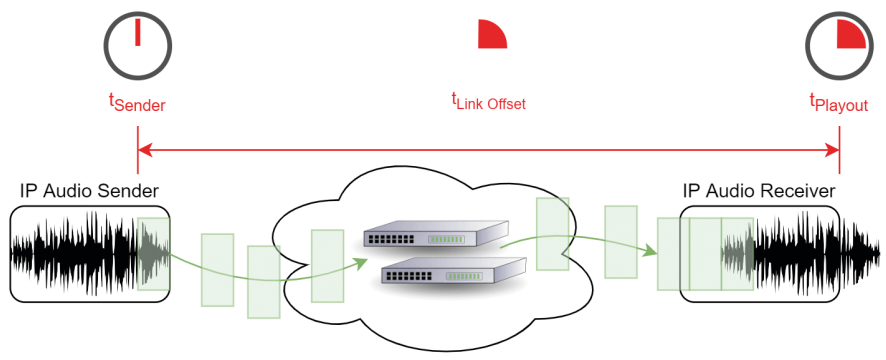
\includegraphics[width=\linewidth, keepaspectratio]{figures/link_offset_latency.png}
	\caption{A kapcsolati eltolás meghatározza a késleltetést \cite{AHNERT2023}}
	\label {fig:link_offset_latency}
\end{figure}
%----------------------------------------------------------------------------
\begin{figure}[H]
	\centering
	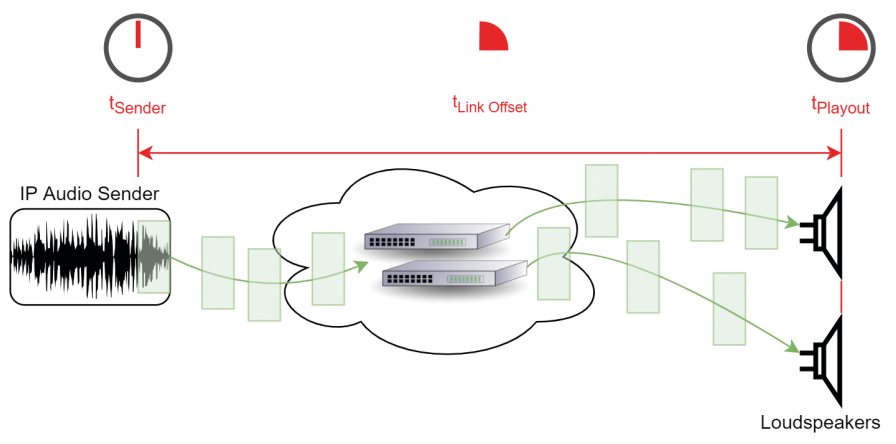
\includegraphics[width=\linewidth, keepaspectratio]{figures/phase_coherence_link_offset.png}
	\caption{Fáziskoherencia azonos kapcsolati eltolással \cite{AHNERT2023}}
	\label {fig:phase_coherence_link_offset}
\end{figure}
%----------------------------------------------------------------------------
\subsection{Szinkronizáció}
%----------------------------------------------------------------------------
Az audiohálózatokban alkalmazott linkeltolást mindig a legnagyobb várható késleltetés alapján 
kell beállítani az összes érintett kapcsolat esetében. Fontos, hogy némi tartalékot is 
hozzárendeljünk a beállított értékhez, amely lehetővé teszi az esetleges, váratlan csomagkiszállítási időingadozások kezelését. 
Ez azt jelenti, hogy a feldolgozási idő átlagánál valamivel hosszabb időkeretet hagyunk. 
Szerencsére ez a megközelítés már széles körben elterjedt, és minden modern audiohálózati szabványban alkalmazásra került.

Az IP alapú küldők és vevők precíz szinkronizációja kulcsfontosságú a minimális késleltetéssel történő működés érdekében. 
A hagyományos audioeszközök esetében ez a szinkronizáció jellemzően különálló word clock kapcsolaton keresztül, 
vagy szinkronizált audioformátumok, például AES/EBU vagy MADI segítségével történt. Ezek a rendszerek egyértelmű 
jelet biztosítottak a mintavételi időpontra vonatkozóan, amely lehetővé tette a vevők számára a frekvencia és 
fázis pontos kinyerését, például analóg-digitális átalakítók esetében.

A PTP (Precision Time Protocol) csomagok kis méretűek, így nem terhelik jelentősen a hálózatot, azonban 
elengedhetetlen, hogy a hálózati eszközökben kiemelt prioritással kerüljenek továbbításra. 
Ez hozzájárul a szinkronizációs pontosság javításához. A QoS (Quality of Service) szabályok keretein belül a 
PTP csomagoknak még magasabb prioritást kell kapniuk, mint a hangátvitel során használt csomagoknak, hogy 
biztosítsák a pontos időzítést az egész hálózatban.

Az összes hálózati eszköz a PTP segítségével egyetlen referenciaidőponthoz igazodik. Ezt az időt egy 
úgynevezett óravezető (PTP leader) eszköz határozza meg, míg a többi eszköz óra követőként szinkronizálódik hozzá. 
Minden eszköz ebből az abszolút időből generálja a saját belső óráját, amit médiaórának nevezünk. 
A gyártóknak gondoskodniuk kell arról, hogy a médiaóra frekvenciája és fázisa pontosan megegyezzen minden eszköz 
esetében, amely a hálózatban működik. Bár technikailag elérhető a magas fokú pontosság, ennek megvalósítása jelentős kihívást 
jelent az audioeszközöket gyártó vállalatok számára. 
A szinkronizáció minősége eszközönként változhat, azonban elfogadhatónak tekinthető, ha a fáziskésés mértéke nem haladja meg az 1 mikroszekundumot.

Mivel az IT-hálózatok nem determinisztikusak a csomagok érkezési idejének tekintetében, az eszközök pontos
szinkronizálása összetett megoldásokat követel meg. 
A PTP követők fő feladata két hatás kompenzálása, amelyek bármilyen hálózat esetén előfordulhatnak:
%----------------------------------------------------------------------------
\subsubsection{Jitter kompenzáció}
%----------------------------------------------------------------------------
A PTP vezető által küldött szinkronizációs üzenetekben szereplő aktuális időt minden követő eszköz 
megkapja egy ismert multicast cím (224.0.1.129) segítségével. A hálózati infrastruktúra és a 
kapcsolók sajátosságai miatt azonban ez az információ nem mindig érkezik meg egyenletes késleltetéssel a vevőkhöz. 
A késleltetés ingadozása a csomag jitter, illetve csomag késleltetési változás (Packet Delay Variation, PDV) 
nevű jelenség, amelyet minden PTP követőnek képesnek kell lennie kompenzálni. 
Az ilyen típusú hálózatokban az audioeszközök jellemzően 1–8 szinkronizációs üzenetet dolgoznak fel másodpercenként, 
ahol a 8-as érték az interoperabilitás biztosítása érdekében van ajánlva.

%----------------------------------------------------------------------------
\subsubsection{Késleltetés mérése}
%----------------------------------------------------------------------------
A „követő” második alapvető feladata a „vezető” és a „követő” közötti csomagkésleltetés mérésére irányul. 
Ez a késleltetés mérés szükséges ahhoz, hogy a vezető által küldött szinkronizációs üzenetekben szereplő időpontok pontosak legyenek. 
A mérés célja annak meghatározása, hogy mennyi időbe telik egy csomag átvitele a hálózaton keresztül, 
beleértve minden hálózati eszközt, mint például kábeleket és kapcsolókat. A vezető és a követő közötti 
kábelhossz és kapcsolók száma nem befolyásolja a mérés eredményét; az egyedüli tényező a végső késleltetési idő. 
A Precision Time Protocol (PTP) esetében a késleltetés minden követő között nanoszekundumos pontossággal egységes kell legyen.

A PTP működéséhez elengedhetetlen, hogy a késleltetés mindkét irányban, tehát a vezetőtől a követőig 
és vissza, konstans és szimmetrikus legyen. A késleltetés mérése a követő által történik, amely a 
késleltetési kérés és válasz üzenetek váltásával történik. Ezt a mérést rendszerint a szinkronizálási 
aránnyal megegyező gyakorisággal végzik.

Mivel a hálózaton több eszköz is képes lehet PTP vezetőként működni, a szabvány előírásokat határoz 
meg a vezető kiválasztására. Ezt az eljárást a Legjobb Mesteróra Algoritmus (Best Master Clock Algorithm, BMCA) szabályozza.

Minden vezetőként potenciálisan alkalmazható eszköznek lehetősége van bejelentő üzeneteket küldeni, 
amelyek tartalmazzák prioritásaikat és oszcillátoruk pontosságát. Az eszközöknek figyelemmel kell kísérniük más 
eszközök bejelentő üzeneteit is. Amennyiben más eszközök által küldött üzenetek jobb minőséget jeleznek, 
az eszköz leállítja a vezetői szerepéről való bejelentkezést. Ha viszont az üzenetek nem mutatnak jobbat, 
az eszköz folyamatosan küldi saját bejelentő üzeneteit, ezzel jelezve, hogy aktív vezetőként működik.

A bejelentő üzeneteket az announce intervallumnak nevezett időközönként küldik ki. 
Ezek az üzenetek funkcionálhatnak „szívverésként” is, amely biztosítja, hogy a jelenlegi mester még mindig működőképes. 
Ha a kapcsolat megszakad, az eszközök várnak egy bizonyos ideig (bejelentő időtúllépés), 
mielőtt újra elküldik bejelentő üzeneteiket, és ismételjük meg a vezető kiválasztási folyamatot. 
A vezetőváltás során a követőknek folytatniuk kell saját oszcillátoruk működését, biztosítva, hogy az audiofolyam ne szakadhasson meg.

A bejelentő üzenetekben két érték található, amelyeket a felhasználó állíthat be: prioritás 1 és prioritás 2. 
Mindkét érték 0 és 255 közötti tartományban változhat, ahol a 0 a legmagasabb prioritást jelöli. 
Ha az egyik eszköz prioritás 1 értéke alacsonyabb, mint más eszközöké, akkor az az eszköz válik a vezetővé. 
A prioritás 2 értéke csak akkor lényeges, ha több eszköz prioritás 1 értéke megegyezik. 
Ez előfordulhat, ha két azonos típusú eszköz ugyanazon prioritás 1 értéket használ. 
Ebben az esetben a prioritás 2 határozza meg a fő vezetőt és a tartalék vezetőt.

Fontos megjegyezni, hogy bizonyos eszközök nem engedélyezik a felhasználó számára a prioritási értékek megadását. 
Ezek az eszközök „Preferált Vezető” megjelöléssel rendelkeznek, és fix értéket használnak, amit a gyártó állít be. 
Ezért lehetséges, hogy egy másik PTP vezető alacsonyabb érték megadásával felülbírálhatja az ilyen eszközt. 
Néhány eszköz támogatja a „Csak Követő” beállítást is, amely esetén az eszköz sohasem próbálja meg átvenni a vezetői szerepet a PTP hálózaton.
%----------------------------------------------------------------------------
\subsection{Mintavételi frekvencia és bitmélység}
%----------------------------------------------------------------------------
Az audio over IP rendszerek megbízható működéséhez elengedhetetlen a megfelelő mintavételi frekvencia és bitmélység pontos meghatározása.

Ezek a paraméterek jelentős hatással vannak az audio minőségére és a hálózati teljesítményre. 
Fontos figyelembe venni a hálózati átviteli kapacitást, valamint az egyes eszközök által támogatott 
maximális mintavételi frekvenciát és bitmélységet. Amennyiben a hálózat nem képes biztosítani a 
szükséges sávszélességet, instabillá válhat, ami hangkimaradásokhoz, megszakadásokhoz, vagy 
legrosszabb esetben a hálózat teljes összeomlásához vezethet.

A gyakran alkalmazott 48 kHz-es mintavételi frekvencia széles hangszalagot biztosít, és 
általában kompatibilis a legtöbb professzionális hangtechnikai alkalmazással. 
Az utóbbi időben egyre nagyobb népszerűségnek örvend a 96 kHz-es mintavételi frekvencia is, amely fokozott 
részletességet és jobb hangminőséget nyújt. Azonban fontos megjegyezni, hogy a 96 kHz-es mintavételi 
frekvencia nagyobb sávszélességet igényel, ami hatással lehet a hálózat teljesítményére.
A sávszélesség kiszámítása a következő képlettel történik:
%----------------------------------------------------------------------------
\begin{equation}
	\label{eq:sávszélesség}
	Sávszélesség igény = MintavételiFrekvencia * BitMélység * CsatornákSzáma
\end{equation}
%----------------------------------------------------------------------------
Ezzel a formulával könnyen és gyorsan kiszámíthatjuk, hogy a rendszerünknek mekkora sávszélességre lesz szüksége.
Tehát ha egy 64x64 csatornás rendszerünk van, 96 kHz-es mintavételi frekvenciával és 24 bites bitmélységgel,
akkor a sávszélességünk a következő lesz:
%----------------------------------------------------------------------------
\begin{equation}
	\label{eq:sávszélesség}
	96000 * 24 * 64 * 2 = 294912000 bit/s = 294,912 Mbit/s (\text{nyers adatfolyam})
\end{equation}
%----------------------------------------------------------------------------
A hálózatunkat nem centizhetjük ki, mindig kell egy bizonyos tartalékot hagyni a hálózatban. A korábbiakban már említett
legalább 30 százalékos túlméretezést érdemes alkalmazni nem csak elméletben hanem gyakorlatban is. 
Tehát a fenti példában a sávszélességünk a következő lesz:
%----------------------------------------------------------------------------
\begin{equation}
	\label{eq:teljes-sávszélesség}
	294912000 bit/s * 1.3 = 383385600 bit/s = 383,3856 Mbit/s (\text{teljes sávszélesség})
\end{equation}
%----------------------------------------------------------------------------
A számítások alapján egy átlagos 1 Gbit/s (1 Gbit/s = 1000 Mbit/s) sávszélességű hálózaton ez a rendszer már megfelelően működhet,
amennyiben kizárólag audio felhasználásra dedikáljuk a hálózatunkat.
A bitmélység a hangsáv digitális reprezentációját határozza meg, és az adatok pontosságát befolyásolja.
Általában 16 vagy 24 bitmélységű rendszerek használatosak az audio over IP területén, de a Dante rendszerek a 
32 bites bitmélységet is támogatják. A 16 bites reprezentáció megfelelő lehet olyan alkalmazásokhoz, ahol a nagy
dinamikatartomány nem kritikus. Ugyanakkor a 24 bites felbontás lehetőséget nyújt a pontosabb és részletesebb hangátvitelhez,
általában zenei stúdiókban és élőzenei környezetekben. 
A 32 bites bitmélység a legmagasabb minőséget biztosítja, de a sokkal nagyobb sávszélesség igénye miatt elsősorban csak
a kiemelten professzionális stúdiókban használják, de általában az esetek többségében
a 24 bites bitmélységű rendszerek bőven tökéletesen megfelelnek.
%----------------------------------------------------------------------------
\subsection{Késleltetés}
%----------------------------------------------------------------------------
Amennyiben egy csomag 1 ms (milliszekundum) hosszúságú hanganyagot tartalmaz, 
a kapcsolat késleltetése mindig meghaladja az 1 ms értéket. 
Először a küldő eszköznek 1 ms-nyi hanganyagot kell pufferelnie, mielőtt 
azt csomagba helyezi és továbbítja a hálózaton. Ezt követi a csomag hálózati 
utazási ideje, amely magában foglalja az összes áthaladási pontot, például kapcsolókat, 
mielőtt a csomag végül elérné a célpont eszköz pufferét.
%----------------------------------------------------------------------------
\begin{enumerate}
    \item Csomag idő
    \item Utazási idő a hálózaton
    \item Fogadási puffer
\end{enumerate}
%----------------------------------------------------------------------------
A gyakorlatban a „link offset” technikai kifejezés azonos jelentéssel bír, mint a késleltetés. A felhasználó feladata, 
hogy olyan link offsetet állítson be, amely biztosítja, hogy a fogadó puffer soha ne ürüljön ki, ezáltal megelőzve a hang megszakadását.
%----------------------------------------------------------------------------
\subsection{IP címek és maszkok}
%----------------------------------------------------------------------------
Egy hálózaton belül minden eszköznek egyedi címre van szüksége ahhoz, hogy a csomagok sikeresen célba érjenek, 
és elkerülhetők legyenek a csomagok ütközései. 
Az egyedi címek lehetnek hardverhez kötődő címek (MAC-címek) vagy konfigurálható címek (IP-címek).
%----------------------------------------------------------------------------
\section{IP-cím hozzárendelési módszerek}
%----------------------------------------------------------------------------
Az IP-címeket háromféleképpen lehet hozzárendelni egy eszközhöz:
%----------------------------------------------------------------------------
\begin{itemize}
    \item \textbf{Felhasználói kézi beállítás:}
    Ez dokumentációt és felhasználói figyelmet igényel annak érdekében,
	hogy egy adott IP-címet csak egyszer használjanak ugyanabban a hálózatban.
	Ez lehet a preferált megközelítés állandó telepítések esetén,
	mivel könnyen tudjuk az IP-címek kiosztásának bizonyos struktúráját követni.
    
    \item \textbf{DHCP szerver általi eszközhöz rendelés:}
    Ez egy rugalmas, mégis strukturált módja az IP-címek elosztásának a hálózaton belül.
	Egy hoszt 'DHCP módban' megpróbálja megtalálni a megfelelő DHCP szervert,
	és minden szükséges IP-konfigurációt egy szabványosított módon szerez be.
	Egy felhasználó ellenőrizheti a DHCP szerverben észlelt eszközöket és azok IP-címeit.
	Az adminisztrátor konfigurálhatja úgy, hogy csak bizonyos IP-cím-tartományt osztanak ki,
	míg másokat kézi rendelésre tartalékolnak.
    
    \item \textbf{Hoszt általi önkiosztással:}
    Ez a mechanizmus még \textit{Zeroconfig} néven ismert, és csak kis telepítésnél
	működik a korlátai miatt, mivel az összes eszköz egy alhálózatban van,
	és nem csatlakozhat más alhálózatokhoz.
\end{itemize}
%----------------------------------------------------------------------------
Egy adott eszköz IP-címének megismerése kihívást jelenthet, ha az nem látható egy kijelzőn. 
Az IP-címek azonosítása és annak meghatározása, hogy két cím azonos alhálózathoz tartozik-e, 
nem lehetséges az alhálózati maszkok ellenőrzése nélkül.

Amennyiben egy csomag cél-IP-címe nem található azonos alhálózaton belül, a küldő eszköznek 
a csomagot a router IP-címére kell irányítania, nem pedig közvetlenül a fogadó eszközhöz.

Az alhálózaton belül a hasonló IP-címek csak az utolsó számjegyekben térnek el egymástól. 
Az IP-cím első része, amely a hálózati címkét jelöli, és a második része, amely a 
hosztcímkét képviseli, az alhálózati maszk segítségével különíthető el. 
Az alhálózati maszkban a 0'-val jelölt pozíciók határozzák meg a hálózati címkét, 
míg a hosztcím a maradék, 0'-val jelölt rész bal oldalán található. 
A hálózati címkét az alhálózati maszkban egy 0'-nál nagyobb érték jelzi, míg a hosztcím a maradék 0'-val jelölt pozíciókban található.
%----------------------------------------------------------------------------
\begin{figure}[H]
    \centering
    \begin{minipage}{0.45\textwidth}
        \centering
        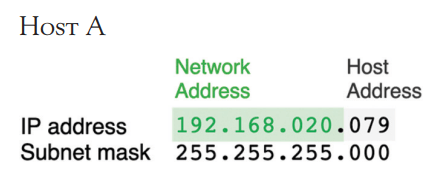
\includegraphics[width=67mm, keepaspectratio]{figures/host_a.png}
        \caption{Host A}
    \end{minipage}\hfill
    \begin{minipage}{0.45\textwidth}
        \centering
        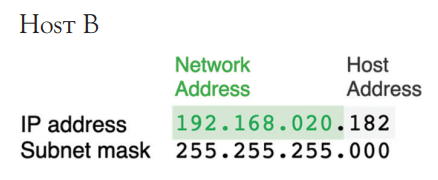
\includegraphics[width=67mm, keepaspectratio]{figures/host_b.png}
        \caption{Host B}
    \end{minipage}
\end{figure}
%----------------------------------------------------------------------------
Host A és Host B ugyanazon alhálózatban találhatóak, mivel mindkettő azonos hálózati címkét használ (192.168.020). 
Az IP-cím hálózati részét az alhálózati maszk 255-ös értéke határozza meg. E két eszköz között tehát nincs szükség routerre.
%----------------------------------------------------------------------------
\begin{figure}[H]
	\centering
	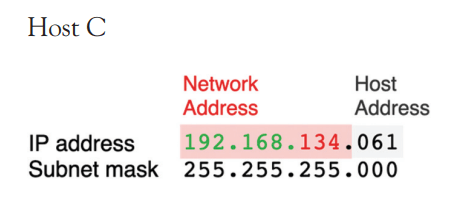
\includegraphics[width=67mm, keepaspectratio]{figures/host_c.png}
	\caption{Host C}
	\label {fig:host_c}
\end{figure}
%----------------------------------------------------------------------------
Host C viszont eltérő alhálózaton helyezkedik el, mivel a hálózati címében eltérés van (192.168.134 a 192.168.020 helyett). 
Ennek következtében Host C nem képes közvetlen csomagcserére Host A-val és Host B-vel router nélkül. 
A kommunikációhoz Host C-nek olyan IP-címet kell kapnia, amely a 192.168.134\ldots tartományba esik, 
vagy az alhálózati maszkot is módosítani kell, például 255.255.0.0-ra.

Az alhálózati maszkok decimális jelölését dot-decimális formátumnak nevezzük. 
Az információk rövidebb jelölésére gyakran alkalmazzák a CIDR (Classless Inter-Domain Routing) 
vagy perjel alapú jelölést. Ez a jelölés az IP-cím után következő perjel után az alhálózati maszkot 0'-nál 
nagyobb értékekkel tünteti fel. A CIDR jelölés az alhálózati maszk bináris formájára utal, 
például a 255' a 11111111'-nek felel meg. A példák alapján az alhálózati maszkok bináris formájukban 24 1'-et tartalmaznak.
A fenti példában szereplő hosztok CIDR jelölése:

%----------------------------------------------------------------------------
\begin{itemize}
    \item \textbf{Host A:} 192.168.020.182/24
    \item \textbf{Host B:} 192.168.020.079/24
    \item \textbf{Host C:} 192.168.134.61/24
\end{itemize}
%----------------------------------------------------------------------------

A routerek alkalmazása során és több alhálózat összekapcsolására szolgáló telepítések az OSI modell harmadik rétegén működnek. 
Ez a modell a hálózati funkcionalitást hét rétegre bontja, ahol mindegyik réteg egy adott 
szolgáltatási készletet határoz meg a hálózati eszközök által biztosított funkciókról. 
A harmadik réteg feladata a csomagok célba juttatása a megfelelő címzett felé.

Az összes modern IT eszköz követi ezt az absztrakciós rétegkoncepciót, amely biztosítja a gyártók 
közötti interoperabilitást. A harmadik réteghez tartozó telepítések képesek az IP-címek és az 
alhálózati maszkok értelmezésére, amely lehetővé teszi a csomagok továbbítását az alhálózatok között. 
Az ilyen típusú technológiák képesek a kívánt működésre. Ezzel szemben bizonyos technológiák csupán a második rétegre korlátozódnak.

Ez azt jelenti, hogy a csomagok továbbítása kizárólag MAC-címek alapján történik, és nem 
tartalmaznak alhálózati információkat. Ennek következtében a második rétegű hálózatokat nem 
lehet több alhálózatra bontani, a csomagok továbbítása nem végezhető routerek által, ami 
jelentős mértékben korlátozza a skálázhatóságot. A második rétegű hálózatok egyik ismert példája a TSN/Milan és a CobraNet.

%----------------------------------------------------------------------------
\begin{figure}[H]
	\centering
	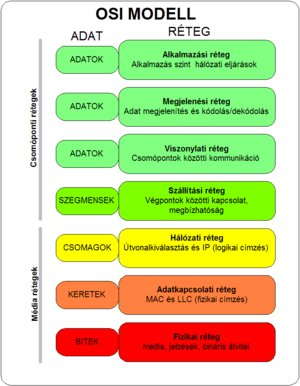
\includegraphics[width=150mm, keepaspectratio]{figures/osi_modell.jpg}
	\caption{Az OSI modell}
	\label {fig:osi_modell}
\end{figure}
%----------------------------------------------------------------------------

Az alhálózat egy logikai egységet jelent egy adott hálózaton belül. 
Az alhálózatok létrehozása többféle célt szolgál, például adminisztratív és biztonsági okokból. 
A routerek feladata az alhálózatok összekapcsolása, lehetővé téve ezzel, hogy a hosztok csomagokat 
cseréljenek anélkül, hogy elhagynák saját alhálózatukat. 
Az alhálózatok közötti forgalom irányításához a megfelelő hálózati útvonalak konfigurálása szükséges.

Ezzel szemben a hagyományos kapcsolók nem képesek alhálózatok összekapcsolására. 
Alternatív megoldásként a virtuális LAN (VLAN) használata lehetővé teszi a hálózat szegmentálását. 
A VLAN létrehozása növeli a rendszer rugalmasságát, és csökkenti a különböző rendszerek közötti felesleges kommunikációt. 
Emellett a VLAN-ok biztonságosabb módot nyújtanak a hosztok egymástól való elkülönítésére, szemben az alhálózatokkal.

%----------------------------------------------------------------------------
\subsection{Hálózati topológiák}
%----------------------------------------------------------------------------
A csomópontok különböző módszerekkel kapcsolódhatnak egymáshoz, és a topológia kiválasztása az 
egyik legfontosabb döntés a hálózat tervezése során. A csillag topológia széles körben 
alkalmazott megoldás, amelyben több hoszt egy központi eszközhöz, például kapcsolóhoz vagy 
routerhez csatlakozik. A modern hálózatok gyakran alkalmaznak kettős csillagtopológiát, 
amelyet gerinc/levél architektúrának neveznek. Ebben a struktúrában a központi eszköz (gerinc) 
általában több adatforgalmat kezel, mint a perifériális eszközök (levél). Amennyiben a 
gerinc és a levél közötti nagy sávszélességű kapcsolat nem képes egyszerre kezelni az 
összes hoszt forgalmát, a rendszer blokkolhat. Az ellentétes megközelítés a nem blokkoló 
hálózattervezés, ahol a nagy sávszélességű kapcsolatok képesek kezelni a hozzájuk csatlakoztatott hosztok teljes forgalmát.

A gyűrű topológia szintén egy népszerű megoldás, amely több interfésszel rendelkezhet. 
A gyűrű topológia megvalósításához legalább két interfész szükséges. 
Minden két csomópont közötti kapcsolat teljes sávszélességet biztosít, és a csomópontok 
feladata a csomagok továbbítása a gyűrűn belül. Ebben a rendszerben minden csomópont 
olyan módon működik, mint egy kapcsoló, amely csomagokat továbbít a két interfésze között. 
A gyűrű topológia gyakran választott megoldás nagy távolságok áthidalására és költséges kapcsolatok esetén. 
Gyakorlati alkalmazásai közé tartoznak a különböző helyszínek közötti hálózatok, illetve olyan 
eszközök összekapcsolása, ahol nincs hely további kapcsolók elhelyezésére. Ezen kívül a gyűrű 
topológiák beépített redundanciát nyújtanak, lehetővé téve a hozzáférést minden eszközhöz még akkor is, ha egy kapcsolat megszakad.

A megfelelő hálózati kialakításhoz alapvető fontosságúak a nem blokkoló kapcsolók is. 
A nem blokkoló architektúra azt jelenti, hogy a kapcsoló nem jelent szűk keresztmetszetet a rendszerben. Ez azt jelenti, hogy képes kezelni az összes rá érkező forgalmat, ahol csupán a port sebessége szabhat határt.

%----------------------------------------------------------------------------
\subsection{Unicast és Multicast} %Egyedi és Csoportos Küldés
%----------------------------------------------------------------------------

Amikor egy eszköz adatcsomagot küld egy másik eszköznek, ezt unicast módszernek nevezzük. 
Ilyenkor a kapcsolatnak pontosan egy küldője és egy fogadója van. 
Az unicast gyakran a Transmission Control Protocol (TCP) segítségével történik, ahol a 
fogadó minden egyes csomag sikeres átvételéről visszaigazolást küld a küldőnek. 
Ha a visszaigazolás nem érkezik meg, a küldő automatikusan újraküldi a csomagot.

Az UDP (User Datagram Protocol) egy alternatív megoldás a TCP-hez képest. 
Az UDP esetében a küldő nem kap visszaigazolást a csomagok megérkezéséről, így bízik abban, hogy 
a csomagok sikeresen eljutnak a fogadóhoz. Ha egy csomag elveszik, annak tartalma is elveszik. 
Ez nem jelenti azt, hogy az UDP kevésbé megbízható, csupán más célokra lett tervezve.

Bár ez meglepő lehet, az UDP gyakran előnyösebb a szakmai audio hálózatokban. 
Az alacsony késleltetés érdekében nem megengedett a csomagok újraküldése, mivel ez időt igényelne, 
ami növelné az általános késleltetést. Az élő audio esetén a csomagvesztés kezelése során a legjobb, 
ha azonnal folytatjuk a következő audio minták lejátszását, anélkül hogy megpróbálnánk helyreállítani 
az elveszett csomagokat. A menedzselhető switchek és végpontok lehetővé teszik a 
csomagvesztések naplózását, így nyomon követhető a hálózat állapota.

Az audio alkalmazások gyakran megkövetelik, hogy egy audio jelet párhuzamosan 
több helyszínre továbbítsanak, például egy mikrofonjelet, amelyet egyszerre továbbítanak a 
front-of-house és a monitoring keverőpultokhoz, esetleg egy harmadik helyszínre, például egy felvevő eszközre is.

Amikor a küldő unicast módban küldi el a csomagokat, az audio jel három külön 
csomagként érkezik azonos tartalommal, de eltérő címzésekkel. Ez felesleges terhelést jelent 
a küldő eszköz számára és sávszélességet foglal el mindhárom célhoz. Az optimalizálás érdekében 
a multicast használata ajánlott. A multicast előnyei közé tartozik a csökkentett processzorterhelés 
a küldő eszközön és az általános forgalom csökkentése a hálózaton. A küldő multicast címekre küldi 
a csomagokat, nem pedig egyedi hoszt címekre. Nem tudja, melyik címzettek kapják meg a csomagokat. 
A multicast címek hasonlóak a rádiófrekvenciákhoz: bárki, aki érdekelt, fogadhatja a tartalmat. 
A küldő csak egyszer helyezi el az audio adatokat egy csomagban, és elküldi egy multicast címre. 
A vevőknek tudniuk kell, melyik multicast címre szeretnének hallgatni. 
A multicast címek nem kapcsolódnak közvetlenül az alhálózatokhoz vagy az IP-címekhez, ezért a 
multicast csomagok áthaladnak az alhálózatokon, hacsak nincsenek elkülönítve VLAN-okon keresztül.

Ha a hálózat nem kizárólag audio jelek továbbítására van tervezve, előfordulhat, hogy olyan 
eszközök is csatlakoznak hozzá, amelyek nem kapcsolódnak az audiohoz. Ennek elkerülésére fontos, hogy 
a multicast forgalom csak az arra érdeklődő hosztokhoz jusson el. Ezt az IGMP snooping 
(Internet Group Management Protocol snooping) használatával lehet megoldani. 
Az IGMP snooping lehetővé teszi, hogy a kapcsolók csak azokon az interfészeken küldjék el a 
multicast csomagokat, ahol az érdeklődő hosztok időszakosan IGMP kéréseket küldenek. 
Ha nincs beérkező kérés, a megfelelő multicast leáll, így elkerülhető a felesleges forgalom. 
Az IGMP snooping hasonló egy zsiliphez, amely alapértelmezetten zárva van, és csak kérésre nyílik meg. 
Erősen ajánlott az IGMP snooping aktiválása minden kapcsolóban egy multicast hálózatban. 
Fontos megjegyezni, hogy egy hálózatban csak egy IGMP Querier lehet aktív, mivel az összes 
többi kapcsoló tőle kapja az információkat. Az IGMP Querier hiányában a multicast forgalom 
broadcastként viselkedhet, ami jelentős felesleges forgalmat eredményezhet.

Összefoglalva, az unicast biztosítja a legjobb késleltetési teljesítményt, és a kapcsolók 
számára a legjobban kezelhető. Ezzel szemben a multicast hatékonyabb sávszélesség-kezelést 
kínál, különösen a csatornaszám és a sávszélesség növekedésével.

%----------------------------------------------------------------------------
\subsection{Eszköz- és Adatfolyam-felfedezés}
%----------------------------------------------------------------------------

Az AES67 audiostandard nem határozza meg, hogyan történik a hálózati eszközök felfedezése, illetve mely 
adatfolyamok érhetők el a hálózaton belül. Jelenleg az ismert technológiák közül mindegyik a Bonjour 
vagy mDNS mechanizmusokra támaszkodik az eszközök közötti értesítések kezelésére.

Az eszközök általában egy fix multicast cím (224.0.0.251) felé küldik az értesítéseket, amelyeket más 
eszközök fogadnak, így tájékozódnak egymás jelenlétéről a hálózaton. 
Ennek a megközelítésnek azonban vannak korlátai: nem működik hatékonyan nagyobb telepítésekben, ahol 
több alhálózat vagy VLAN van jelen. Ezen kihívások kezelésére a gyártók saját megoldásokat 
fejlesztettek ki, mint például az Audinate Dante Domain Manager, vagy az audio/video NMOS 
szabványt alkalmazzák a felfedezés és a kapcsolatkezelés érdekében.

Az audio adatfolyamok felfedezése gyártónként eltérő mechanizmusokat használ. Mindkét esetben 
előre meghatározott multicast címek segítségével terjesztik az adatfolyamokkal kapcsolatos 
információkat, lehetővé téve, hogy a címzettek megtalálják az elérhető adatfolyamokat és azok paramétereit:

%----------------------------------------------------------------------------
\begin{itemize}
	\item Session Announcement Protocol (SAP) - minden Dante termék által használt (Multicast cím: 239.255.255.255)
\end{itemize}

\begin{itemize}
	\item Bonjour / mDNS - minden más technológiában használt (Multicast cím: 224.0.0.251) 
\end{itemize}
%----------------------------------------------------------------------------
Szerencsére a mai modern eszközök többsége támogatja mindkét protokoll egyidejű aktiválását, 
ami lehetővé teszi, hogy egy adott audio adatfolyam párhuzamosan áramoljon mindkét mechanizmuson keresztül.

%----------------------------------------------------------------------------
\subsection{Redundancia}
%----------------------------------------------------------------------------
Az audiohálózatok korai fejlődési szakaszaiban bizonyos felhasználók kétségeiket 
fejezték ki az IT hardverek megbízhatóságával kapcsolatban. 
Azonban az elterjedt IT-berendezések nemcsak hogy jól teljesítettek, 
hanem gyakran megbízhatóbbak voltak, mint a hagyományos audioberendezések. 
Ezen kívül a legtöbb IT-hálózati komponens rendelkezik különféle diagnosztikai 
mechanizmusokkal, amelyek lehetővé teszik a berendezések hibáinak gyors azonosítását és orvoslását.

%----------------------------------------------------------------------------
\subsubsection{Spanning Tree Protocol (STP)}
%----------------------------------------------------------------------------
Amennyiben a kapcsolókat olyan módon kötik össze, hogy hurkot képezzenek, 
fennáll a kockázata annak, hogy a csomagok végtelen ciklusban áramlanak a hurokban. 
Ezt a 'visszacsatoló hurok' jelenséget a hálózati hardver automatikusan 
észleli az STP (Spanning Tree Protocol) segítségével. Ha a rendszer hurkot 
érzékel, a kapcsoló automatikusan deaktiválja az egyik kapcsolatot. 
Az STP emellett felhasználható a rendszer véletlenszerű kapcsolatvesztések, például kábelvágások ellen is.

A rendszer úgy van megtervezve, hogy szándékosan hoz létre hurkokat, 
majd ha egy kábel véletlenül kioldódik, azonnal észleli a problémát és 
újraaktiválja a passzív kapcsolatot. Ez a folyamat néhány másodpercet 
vesz igénybe, amely alatt az audio jel rövid időre megszakadhat, de ez 
lényegesen gyorsabb megoldás, mint a manuális hibakeresés és új kábel telepítése. 
A legtöbb rendszerben az STP alapértelmezés szerint engedélyezve van, ami 
elkerüli a broadcast 'viharok' kialakulását, amelyek jelentősen csökkenthetik a 
sávszélességet és túlterhelhetik a hálózatot.

%----------------------------------------------------------------------------
\subsubsection{Link Aggregáció}
%----------------------------------------------------------------------------
Ha egy adott kapcsolat kiemelkedő fontossággal bír egy telepítés során, lehetőség 
van arra, hogy két vagy több kábelt párhuzamosan csatlakoztassunk a biztonság érdekében. 
Habár a link aggregáció elsődleges célja a két kapcsoló közötti sávszélesség növelése, 
ez a megközelítés költséghatékony megoldást kínál a kapcsolat véletlen leválasztásának 
vagy kábelvágásának elkerülésére is. Például egy színpad esetében, amely egy keverőhöz 
csatlakozik, gyakran alkalmazzák ezt a módszert.

A link aggregáció során a kapcsolóknak mindkét végén azonos 
konfigurációt kell alkalmazni: két vagy több interfészt kell Link Aggregációs Csoportként 
kijelölni, amelyek így egyetlen interfészként jelennek meg a kapcsolón. Gyakorlatilag a link 
aggregáció rendkívül hasznos lehet a kábelproblémák csökkentésében. 
Az egyszerűsége miatt csupán egy további kábelt kell biztosítani, és a 
kapcsolók konfigurációját mindkét végén megfelelően be kell állítani.

Ugyanakkor, ha egy kábel lekapcsolódik, előfordulhat, hogy az audioátvitel néhány másodpercig megszakad, 
amíg a kapcsoló az alternatív kapcsolatot aktiválja.
%----------------------------------------------------------------------------
\subsubsection{ Adatfolyam redundancia}
%----------------------------------------------------------------------------
A redundancia biztosítása egy hálózaton belül a legnagyobb biztonságot nyújtó, ám 
legdrágább megoldás az, ha két teljesen független audiohálózatot alakítanak ki. 
Ez a megközelítés két különböző utat biztosít a küldő és a fogadó között. 
Az ilyen rendszerben minden csomópontnak két hálózati interfészt kell rendelkezésre bocsátania.

A küldő fél két, azonos audio tartalommal rendelkező csomagot generál, és mindkettőre 
egyazon PTP-időbélyegzőt helyez el, majd ezeket párhuzamosan továbbítja mindkét hálózaton. 
A fogadó végén mindkét csomagot fogadják és feldolgozzák. Ha az egyik csomag 
esetleg elveszik, a megmaradt csomag még így is tartalmazza az összes szükséges információt, 
biztosítva ezzel, hogy az audiofolyamat zavartalanul folytatódjon.

Ez a módszer egyedülálló módon képes kompenzálni a véletlenszerű csomagvesztést 
egy hálózatban anélkül, hogy újraküldést igényelne a küldőtől, ezzel elkerülve a rendszer késleltetését.
%----------------------------------------------------------------------------
\section{AES67}
%----------------------------------------------------------------------------
Az AES67 szabvány szerint az összes eszköznek meg kell felelnie az
alábbi minimális specifikációknak: 

%----------------------------------------------------------------------------
\begin{itemize}
	\item Unicast és multicast támogatása
	\item UDP/RTP protokollok használata
	\item DSCP címkék beállítása meghatározott értékekre,QoS támogatás 
	\item Nincs meghatározott automatikus eszköz- és adatfolyam-felfedezés 
	\item PTPv2 szabvány használata az időszinkronizációhoz
	\item PTP profil Standard (a gyakorlatban a Dante jelenleg magasabb szinkronizációs rátát igényel)
	\item Küldőknek ki kell adniuk egy SDP fájlt
	\item A fogadóknak érteniük kell egy SDP fájlt
	\item A fogadó puffernek legalább 3 ms hangot kell tudnia tárolni
	\item Adatfolyam formátumok
	\item Egytől nyolc csatorna (a küldő választhat egy fix számot, de a fogadóknak képesnek kell lenniük rugalmasan fogadni bármelyik lehetőséget).
	\item 24 bites és 16 bites felbontás (a küldő választhat egyet, de a fogadóknak mindkettőt érteniük kell) 
	\item 48 kHz mintavételi frekvencia 1 ms csomagidő (48 minta)
	\item A multicast címek 239.0.0.0 és 239.255.255.255 között vannak 
\end{itemize}

A szabványban sok további paraméter és érték szerepel, de ezek nem szerepelnek a
fent felsorolt minimális követelmények között.



% 🚩✋🏻🛑⛔️



%----------------------------------------------------------------------------
\section{Audinate Dante}
%----------------------------------------------------------------------------
\subsection{A Dante hálózatok áttekintése}
%----------------------------------------------------------------------------
A 2020 - 2021-es Covid-19 járvány alatt lehetőségem volt egy széleskörű Dante
kurzusra beiratkozni, amelyet a Dante gyártója, az Audinate szervezett. A kurzus
egy átfogó mély áttekintést nyújtott a Dante hálózatokról. Ebben a fejezetben
fő forrásomnak a belsős oktatóanyagot fogom használni, amelyet a kurzus
során kaptam, pontos és részletes információkat nyújtva a Dante hálózatokról.
Ezek a dokumentumok csak azok számára elérhetőek, akik részt vettek a kurzuson, ebből kifolyólag nem publikusak.

A Dante hanghálózatok digitális hanghálózati technológiát képviselnek, amely
lehetővé teszi a hang elosztását és útválasztását a szabványos Ethernet
hálózatokon keresztül. Az ausztrál Audinate vállalat fejlesztette ki a Dante-t,
amely a szabványos Internet Protocol (IP) hálózatokat használja a magas minőségű,
alacsony késleltetésű hangátvitelhez eszközök között. Ez lehetővé tesz
nagyobb rugalmasságot és skálázhatóságot a hagyományos analóg hangrendszerekhez
képest, valamint biztosítja a hangrendszer integrálását egy meglévő IT infrastruktúrába.
A Dante hanghálózatokat széles körben alkalmazzák, ideértve a koncerthangosítást,
rádiózást, stúdiófelvételeket, vállalati és konferenciaközpontokat, és még sok mást.
A technológia támogat számos hangformátumot és mintavételi rátát, és lehetővé
teszi akár több száz hangcsatorna egyidejű átvitelét egyetlen hálózaton keresztül.
Emellett a Dante hanghálózatok távolról is vezérelhetők és monitorozhatók,
megkönnyítve a nagy, összetett hangrendszerek beállítását és kezelését.

%----------------------------------------------------------------------------
\subsection{Dante hálózatok technikai részletei}
%----------------------------------------------------------------------------
A Dante hanghálózatok két fő komponensből állnak: Dante eszközökből
és Dante hálózatokból. A Dante eszközök olyan hangeszközök, amelyeket
kifejezetten a Dante protokollhoz terveztek, mint például hangkártyák, erősítők
és hangládák. Ezeket az eszközöket szabványos Ethernet kábelekkel és
kapcsolókkal lehet csatlakoztatni a Dante hálózathoz.
A hálózatot az Audinate Dante Controller szoftverrel lehet
konfigurálni, amely lehetővé teszi a hang elosztását és útválasztását az
eszközök között. A szoftverrel tudjuk az eszközöket távoli vezérléssel elérni és
monitorozni a hálózaton. Ezek a hanghálózatok támogatnak számos
hangformátumot és mintavételi rátát, és képesek egyszerre több száz hangcsatorna
átvitelére egyetlen hálózaton keresztül. A technológia továbbá támogat olyan
fejlett funkciókat, mint a Dante Domain Manager (DDM) a biztonságos
hangátvitelhez, valamint a Dante Virtual Soundcard (DVS) a számítógépes alapú
hanglejátszáshoz és felvételhez. 

Tegyük fel, hogy több eszköz is küld hangot egy adott végpontra a hálózaton.
Alapesetben, ahogy a csomagok felgyülemlenek, az elsőként érkezőket, elsőként szolgálják ki elvet alkalmazzák.
A Dante hanghálózatok Quality of Service (QoS)
támogatást is nyújtanak, a prioritások kezelésére.
Ezzel biztosítható a hangátvitel elsőbbse más hálózati forgalommal szemben. Ez segít minimalizálni a hálózati
torlódás lehetőségét és biztosítani, hogy a hangátvitel minimális késleltetéssel
és magas minőségben történjen. 
Körülbelül 70 százalékos hálózati szaturációnál már ajánlott a QoS használata.
Valamint 100 Mbps-es hálózatoknál segít a jitter csökkenésében.

%----------------------------------------------------------------------------
\subsubsection{Több mintavételi ráta és bitmélység}
%----------------------------------------------------------------------------

A rendszer képes egyidejűleg több bitmélységet kezelni. Ennek informatikai háttere a
a következő képpen néz ki. Ha egy 32 bites hangforrásunk van, de a másik eszköz
csak 24 bites hangot tud fogadni, akkor a Dante a 32 bites hangot 24 bitesre tudja 
alakítani.

%----------------------------------------------------------------------------
\begin{align*}
	\begin{array}{|c|c|}
	\hline
	\text{Hangminták} & \text{Bitmélység} \\
	\hline
	\text{11110000 11110000 11110000 11110000} & \text{32 bites} \\
	\hline
	\text{11110000 11110000 11110000} & \text{24 bites} \\
	\hline
	\end{array}
\end{align*}
%----------------------------------------------------------------------------
	
Amint a példában látszik, 32 bites hangból úgy kaptunk 24 bites hangot, 
hogy egyszerűen csak elhagytuk az utolsó 8 bitet. Ez a folyamat visszafelé is működik,
ha 24 bites hangot kell 32 bites hanggá alakítani, akkor az utolsó 8 bitet 0-val kell feltölteni.

%----------------------------------------------------------------------------	
\begin{align*}
	\begin{array}{|c|c|}
	\hline
	\text{Hangminták} & \text{Bitmélység} \\
	\hline
	\text{11110000 11110000 11110000} & \text{24 bites} \\
	\hline
	\text{11110000 11110000 11110000 00000000} & \text{32 bites} \\
	\hline
	\end{array}
\end{align*}
%----------------------------------------------------------------------------

Mintavételezési frekvencia eltérést csak abban az esetben tudja kezelni, ha a
bitmélység is eltérő. Amennyiben a bitmélység azonos, de a mintavételezési
frekvencia eltérő, akkor a rendszer nem képes a hangot továbbítani.
Ez a mechanizmus egy egyszerű mechanikai példával jól megérhető és leírható.
Tegyük fel van két fogaskerekünk. Amennyiben a mintavételezési frekvencia azonos, és a 
bitmélység eltérő, akkor a fogaskerekek egymásba illeszthetőek és csak a fogaskerekek
mélysége fog eltérni. Amennyiben a mintavételezési frekvencia eltérő, akkor a fogaskerekek
nem illeszthetőek egymásba, és nem tudjuk továbbítani a hangot. Ebben az esetben már egy
konverterre lesz szükségünk, amely képes a két fogaskereket összeilleszteni számunkra.
Egy fontos kitétel van ahhoz, hogy a több mintavételi ráta egyszerre megfelelően működjön,
az pedig az egységes órajel az összes mintavételi frekvenciához.

%----------------------------------------------------------------------------
\subsubsection{Hálózati topológiák}
%----------------------------------------------------------------------------
A Dante rendszerek alapvetően kétféle módban tudnak üzemelni. Az első a
switched (kapcsolt) mód, amelyben az eszközökön található két Ethernet port
egy hálózatot alkot. Ebben a módban tudunk Daisy Chain (füzéres) topológiát kialakítani,
amelyben az egyik eszköz a másikhoz csatlakozik, és így tovább. Továbbá csillagtopológiát
is kialakíthatunk, amelyben minden eszköz egy központi kapcsolóhoz csatlakozik.
%----------------------------------------------------------------------------
\begin{figure}[H]
	\begin{minipage}{0.5\textwidth}
		\centering
		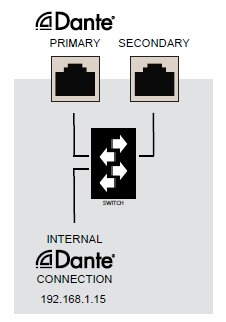
\includegraphics[width=100px, keepaspectratio]{figures/dante-switched-mode.jpg}
		\caption{Kapcsolt mód}
		\label{fig:dante_switched}
	\end{minipage}%
	\begin{minipage}{0.5\textwidth}
		\centering
		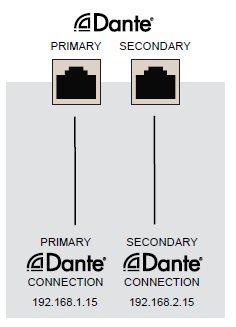
\includegraphics[width=100px, keepaspectratio]{figures/dante-redundant-mode.jpg}
		\caption{Redundáns mód}
		\label{fig:dante_redundant}
	\end{minipage}
\end{figure}

%----------------------------------------------------------------------------
A másik mód a redundant (redundáns) mód, amelyben az eszközökön található két
Ethernet port két különálló hálózatot alkot. Ebben a módban a hálózat redundáns
kialakítású, és a hálózat egyik része automatikusan átveszi a másik rész szerepét,
ha az meghibásodik.
Néhány Dante eszköznek létezik egy harmadik Ethernet portja, amelyet konfigurálási
és vezérlési célokra használnak.
%----------------------------------------------------------------------------
\subsubsection{Késleltetés}
%----------------------------------------------------------------------------
A késleltetés az az idő, amely szükséges egy folyamat végrehajtásához. Például
az idő amíg a bemeneti oldalon egy hangjel feldolgozásra kerül, és a kimeneti
oldalon megjelenik. 
Két fő mértékegységet használunk a késleltetés mérésére:
%----------------------------------------------------------------------------
\begin{equation}
	\label{eq:milliseconds}
	1 \text{ másodperc} = 1000 \text{ milli másodperc}, \quad \text{azaz} \quad 1 \text{ ms} = 0.001 \text{ s}
\end{equation}
%----------------------------------------------------------------------------
%----------------------------------------------------------------------------
\begin{equation}
	\label{eq:microseconds}
	1 \text{ másodperc} = 1000000 \text{ mikro másodperc}, \quad \text{azaz} \quad 1 \mu\text{s} = 0.000001 \text{ s}
\end{equation}
%----------------------------------------------------------------------------
A Dante eszközök lehetővé teszik a késleltetés teljesítményének meghatározását. 
A 0.1 milliszekundumos késleltetés az a késleltetés, amely már kapcsoló lépés biztos.
Ha két eszköz különböző késleltetésű, akkor a nagyobb érték lesz az irányadó.
Egy megfelelően konfigurált modern Dante hálózatban a késleltetés 1 ms körüli értéket vesz fel.
Ez azt is jelenti, hogy például egy dobos előbb hallja a hangszerét a fülmonitoron, mint a saját dobját.

%----------------------------------------------------------------------------
\subsubsection{Órajel}
%----------------------------------------------------------------------------

Minden eszköz egy nagyon-nagyon pontos Dátum/Idő órát követ.
Szinkronizálnak az időhöz és állítják a sebességet, hogy egységes legyen.
Mi a helyzet a terjedési késéssel? Miért vannak szinkronban a Dante eszközök?
A PTP (Precision Time Protocol) késleltetési kéréseket (Delay Requests)
ad ki, amelyek kiszámítják a hálózat késleltetését. 
Az eszközök az információváltás késését is kompenzálják.
A Dante automatikusan választ óra vezetőt.
Mindig csak egy óra vezető lesz, függetlenül a mintavételi rátától.
Beállíthatunk külső óra vezetőt is amennyiben szükséges.
Nem szinkronizál újra, hanem beállítja a sebességet és kompenzálja a hálózati késést.
A Dante által végzett tesztelések és tapasztalatok alapján
bebizonyosodott, hogy az időzítés szinkronban marad akkor is,
ha az óra perceken keresztül teljesen eltűnik.

%----------------------------------------------------------------------------
\begin{figure}[H]
	\centering
	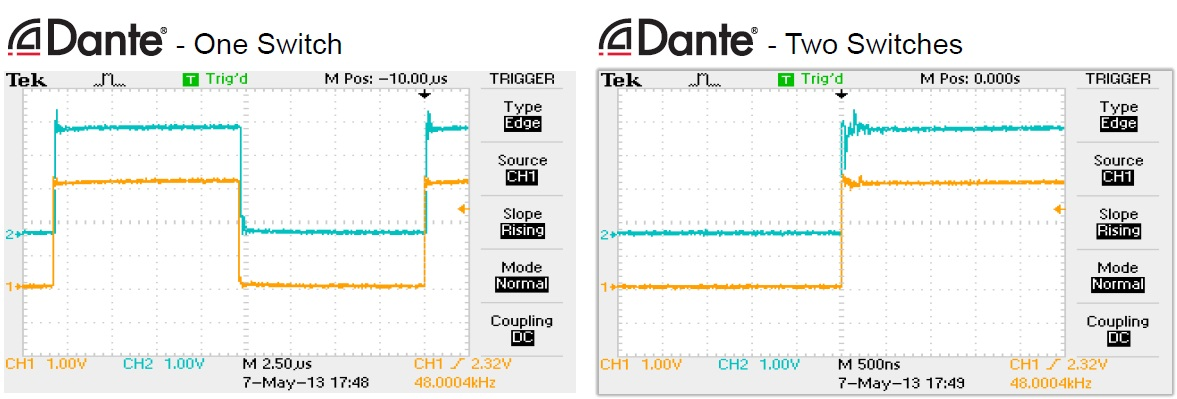
\includegraphics[width=400px, keepaspectratio] {figures/dante-clocking.jpg}
	\caption{Dante órajel}
	\label{fig:dante-clock}
\end{figure}
%----------------------------------------------------------------------------

%----------------------------------------------------------------------------
\subsection{Összehasonlítás a hagyományos hangrendszerekkel}
%----------------------------------------------------------------------------
A hagyományos hangrendszerek általában analóg kábelekre és csatlakozókra
támaszkodnak a hangjelek eszközök közötti átviteléhez. Ezek a rendszerek
korlátozottak lehetnek rugalmasságban, skálázhatóságban és az egyidejűleg
átvihető hangcsatornák számában. Emellett hajlamosak bonyolultabbá válni a
beállítás és kezelés szempontjából, mivel minden hangcsatornához külön kábel és
csatlakozás szükséges. A Dante hanghálózatok jóval több hangcsatornát is támogatnak,
mint a hagyományos analóg rendszerek, lehetővé téve a nagy, összetett hangrendszerek könnyű
beállítását és kezelését. A Dante hanghálózatok további előnye, hogy képesek
hangot továbbítani hosszú távolságokon anélkül, hogy a minőség romlana. A
hagyományos analóg rendszerek zajra és jelveszteségre hajlamosak hosszú kábelek
esetén, míg a digitális hangjelek, amelyeket az Ethernet hálózatokon
továbbítanak, minimális minőségveszteséggel juthatnak el nagy távolságokra.
%----------------------------------------------------------------------------
\begin{table}[htbp]
    \centering
    \caption{Digital Snake és DigitalAVNetwork Jelút opciók}
    \begin{tabular}{@{}lll@{}}
        \toprule
        \textbf{Kérdés} & \textbf{Pont-pont között} & \textbf{Hálózati megoldás} \\ \midrule
        Hová megy a jel? & Lineáris kábelút & Bárhol a hálózaton \\
        Hogyan változtassuk meg a jelútvonalat? & Mozgassuk a kábelt & Egy egérkattintással \\
        Szétválaszthatjuk-e a jeleket? & Nem & Igen - a hálózaton \\
        Megosztható-e a kábel más jelekkel? & Nem & Igen - közös infrastruktúra \\
        \bottomrule
    \end{tabular}
    \label{tab:digital-snake-vs-digitalavnetwork-hu}
\end{table}
%----------------------------------------------------------------------------
\begin{figure}[H]
	\centering
	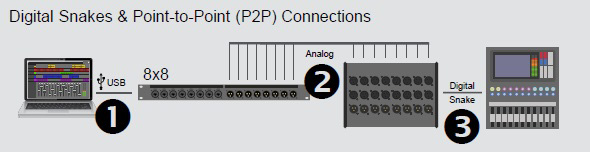
\includegraphics[width=\linewidth, keepaspectratio]{figures/dsnake-p2p.jpg}
	\caption{Digital Snake és Pont-pont közötti (P2P) kapcsolatok}
	\label {fig:dsnake-p2p}
\end{figure}
%----------------------------------------------------------------------------
\begin{figure}[H]
	\centering
	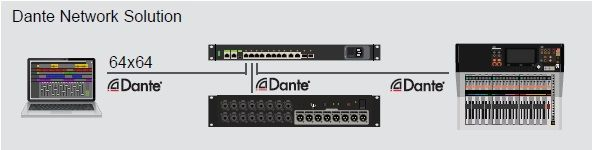
\includegraphics[width=\linewidth, keepaspectratio]{figures/dante-solution.jpg}
	\caption{Dante hálózati megoldás}
	\label {fig:dante-solution}
\end{figure}
%----------------------------------------------------------------------------

A rugalmasság és a skálázhatóság tovbbi kulcsfontosságú előnye a Dante
hanghálózatoknak a hagyományos analóg hangrendszerekkel szemben.
Képesek alkalmazkodni különböző hangkonfigurációkhoz és követelményekhez. 
Könnyű eszközöket hozzáadni vagy eltávolítani, megváltoztatni a hangjelek útvonalát, és a rendszert újra
konfigurálni szükség esetén. Ez lehetővé teszi testreszabott audio-megoldások
létrehozását, amelyeket az adott alkalmazás vagy környezet speciális igényeihez
lehet igazítani. 

%----------------------------------------------------------------------------
\subsection{Firmware frissítés}
%----------------------------------------------------------------------------

A Dante eszközök rendelkeznek Dante Firmware és Eszköz Firmware-el.
Lehet, hogy mindkettőt frissíteni kell. Kérjük, forduljon a gyártóhoz a párosított verziókért.
Néhány eszköz sorozat más módszerekkel frissíthető.
A Dante Updater hasznos lehet a frissítések nyomon követéséhez és telepítéséhez.
A rendszer ellenőrzi az online adatbázisunkat, hogy tájékoztassa Önt az elérhető frissítésekről.
A Dante firmware könnyen frissíthető.
A Dante Firmware Update Manager továbbra is aktuális.
Importálja a firmware fájlokat, ha firmware-t kap egy gyártótól.
Ha a frissítés nem sikerül, rendelkezünk vészhelyzeti helyreállítási módszerrel.
A Dante eszközök erős támogatást nyújtanak a vegyes firmware verziókhoz.
Mérnökeink automatizált regressziós tesztelést végeztek a korábbi firmware kiadásokkal szemben.

%----------------------------------------------------------------------------
\subsection{Chipek}
%----------------------------------------------------------------------------

A Dante hálózatok változatos chipekkel építhetők fel. 
Az Audinate számos különböző chipet kínál a Dante hálózatok létrehozásához, 
melyek eltérő hangcsatorna-számot és egyéb funkciókat támogatnak. 
A Dante chipek különféle méretekben és árkategóriákban elérhetők, 
lehetővé téve a gyártók számára, hogy különféle méretű és árú Dante 
eszközöket fejlesszenek ki, így képesek kielégíteni a különböző piaci igényeket. 
A Dante chipek segítik a gyártókat abban, hogy gyorsan és hatékonyan hozzanak 
létre Dante-kompatibilis eszközöket, és könnyedén integrálják azokat a saját termékeikbe.

%----------------------------------------------------------------------------
\begin{center}
	\begin{tabular}{|c|p{10cm}|}
		\hline
		\textbf{Chip} & \textbf{Leírás} \\
		\hline
		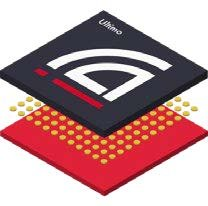
\includegraphics[width=40px,height=40px,keepaspectratio]{figures/ultimo-x.jpg} & \textbf{Dante Ultimo-X} - 0x4, 2x2, 4x0 \\
		\hline
		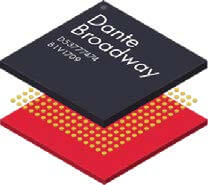
\includegraphics[width=40px,height=40px,keepaspectratio]{figures/broadway.jpg} & \textbf{Dante Broadway} - 16x16 \\
		\hline
		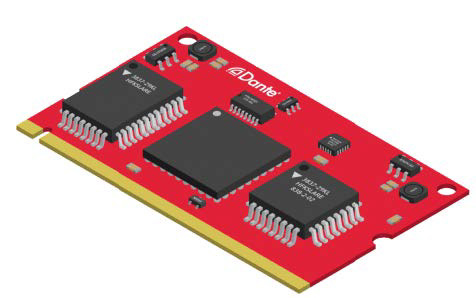
\includegraphics[width=40px,height=40px,keepaspectratio]{figures/brooklyn-ii.jpg} & \textbf{Dante Brooklyn II} - 64x64 \\
		\hline
		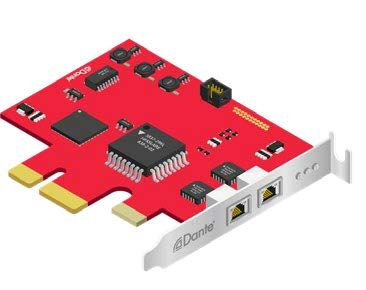
\includegraphics[width=40px,height=40px,keepaspectratio]{figures/pcie-r.jpg} & \textbf{Dante PCIe-R} - 128x128 \\
		\hline
		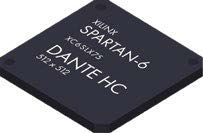
\includegraphics[width=40px,height=40px,keepaspectratio]{figures/dante-hc.jpg} & \textbf{Dante HC (High Capacity)} - 512x512 \\
		\hline
		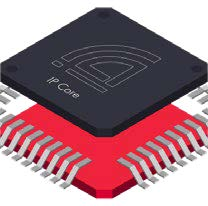
\includegraphics[width=40px,height=40px,keepaspectratio]{figures/shared-processor.jpg} & \textbf{Dante Shared Processor} - IP Core 512x512 FPGA and Dante Embedded Platform 64x64 X86/ARM \\
		\hline
		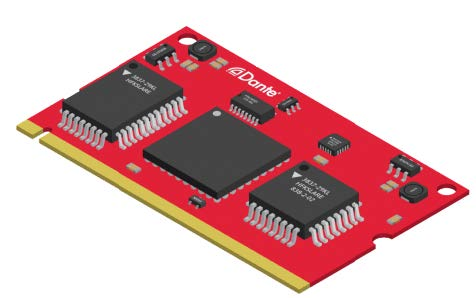
\includegraphics[width=40px,height=40px,keepaspectratio]{figures/dante-av.jpg} & \textbf{Dante AV} - V:1, A:8 \\
		\hline
	\end{tabular}
\end{center}
%----------------------------------------------------------------------------
	






